%!TEX root = tesi.tex


\chapter{ \bfseries Three dimensional dualities}
\section[Susy field theories in 3D]{Supersymmetric field theories in three dimensions}
Spinors in three dimensions have different properties than their four dimensional counterpart.\\
The dimension of the representation in an arbitrary dimension $D$  is given by $2^{\frac{D}{2}} $
for $D$ even, while $2^{\frac{D-1}{2}} $ for $D$ odd.
Hence, in three dimension we have a two dimensional representation.
In odd dimensions representations are irreducible and Weyl spinors do not exist: the chirality operator ($\gamma_{D+1}$ or $\gamma^*$ ) is proportional to the identity.
\\
%This is related to the fact that representations in odd dimensions are constructed by taking the representation in one dimension less, which is even, and adding the chirality operator as the $D$-th matrix in the Clifford algebra.\\
Gamma matrices can be chosen real and the Majorana condition can be imposed, lowering the degrees of freedom of the representation from four to two.\\
Since $3d \; \mN=2$ theories have four supercharges, we can use the $4d \; \mN=1$ superspace formalism. 
\\
The supersymmetry algebra and its representations can be found by dimensional reduction from four dimensions. 
The reduced algebra reads
\begin{equation}
 \{ Q_{\alpha},Q_{\beta} \} =  \{ \bar{Q}_{\alpha},\bar{Q}_{\beta} \}= 0 \qquad \{ Q_{\alpha} , \bar{Q}_{\beta}   \} = 2 \sigma^{\mu}_{\alpha \beta} P_{\mu} + 2 i \epsilon_{\alpha \beta} Z
 \end{equation} 
 where 
The central charge $Z$ is the component of the momentum  along the reduced direction.
Because of the presence of the central charge in the algebra, now states must satisfy a BPS bound of the form $M \geq Z $, which implies that massless representations have null central charge.
\\
The automorphism of this algebra is $U(1)_R \simeq SO(2)_R$, as in four dimensions.
\\
Superspace formalism is similar to what we introduced previously, with proper changes due to the different spinor representations in three dimension such as gamma matrices.
\\
Chiral superfields contain \emph{on-shell} one complex scalar and a complex spinor as in four dimensions.\\
A Vector superfield contains an additional real scalar field with respect to the four dimensional superfield.
The scalar $\sigma $ comes from the component of the four dimensional vector field $A_{\mu}$ along the reduced direction.









\subsubsection{Coulomb branch and dualized photon	}

%%%%% Devo far passare il messaggio che FI è carica di U(1)_J
In three dimensions a free photon can be dualized to a scalar $\gamma$ since it has only one polarization.
Instead of defining a potential $A$ in order to solve the Bianchi identity $d F = d^2 A = 0$, we can define a scalar such that
\begin{equation}
  * F = \frac{g^2}{\pi} d  \gamma  \quad \rightarrow \quad d * F  = 0  
\end{equation} 
\begin{comment}
\begin{equation}
  \epsilon_{\mu \nu \rho} F^{\nu \rho} = \frac{g^2}{\pi} d_{\mu}  \gamma  \quad \rightarrow \quad d * F  = 0  
\end{equation} 
\end{comment}
where 
$*$ is the Hodge operator \footnote{
  The Hodge operator acts on $p$-forms in a $n$ dimensional manifold.
  For a $p$-form $\omega$ its action is given by 
  $$
    ( * \omega)_{\mu_1 \dots \mu_{n-p}} = \frac{\sqrt{g}}{p!} \epsilon_{\mu_1 \dots \mu_n} g^{\mu_{n-p+1} \nu_1 \dots \mu_{n} \nu_p } \omega_{\mu_1 \dots \mu_p}
  $$
}
and 
$g$ is the gauge coupling.\\
The Bianchi identity $d F = 0$ can be seen as a conservation law for the topological current, which is defined as
\begin{equation}
 J_{\mu}^{top} = \frac{1}{2 \pi} ( * F)_{\mu} \; =  \; \frac{1}{2 \pi} d \, \gamma \qquad \partial^{\mu} J_{\mu} =0
\end{equation}
The topological current acts as shifts of the dualized photon $\gamma \rightarrow \gamma + \alpha$.\\
The quantization of the magnetic flux implies that the dualised photon is periodic and is normalized in such a way that $\gamma \sim \gamma + 2 \pi$.
\\
From a vector superfield $V$ we can define a linear multiplet $\Sigma$, given by
\begin{equation}
 \Sigma = \epsilon^{\alpha \beta} D_{\alpha} D_{\beta} V
 \label{eqn:linear_multiplet_gauge}
\end{equation}
It satisfies $D^2 \Sigma = 0$ and is gauge invariant under a transformation $V \rightarrow V + i (\Phi - \Phi^{\dagger})$.
The lowest component of $\Sigma$ is the scalar in the vector multiplet.
It contains also a term $ \bar{\theta} \sigma_{\rho} \theta \, \epsilon^{\mu \nu \rho} F_{\nu \rho}$,which is proportional to the topological current.
The super Yang-Mills action can be written as
\begin{equation}
S \sim \int d^4 \theta \; \Sigma^2
\end{equation}
The  vacuum expectation values of scalar fields in the vector multiplet parametrize a subset of the moduli space of the theory which is called the \emph{Coulomb branch}.
Using the dualized photon we can turn the vector multiplet into a chiral multiplet, whose lowest component is a good parametrization of the Coulomb branch 
\begin{equation}
 Y = \exp{ \left( \frac{2 \pi \sigma}{g^2} + i \gamma \right)}
\end{equation}
because of its periodicity, it's natural to assign $\gamma$ to a phase factor.\\
The classical lagrangian term of matter multiplets in representations $R_f$ of the gauge group is
\begin{equation}
\sum_f \int d^4 \theta Q^{\dagger}_f  e^{V} Q_{f}
\end{equation}
The dualization of the photon is possible as long there is no matter in the theory.\\
The expansion of $V$ contains a term $\sigma \theta \bar{\theta}$ which give rise to a potential term for the squarks of the form
\begin{equation}
\sum_f | \sigma Q_f|^2
\end{equation}
As a result, matter fields couple with $\sigma$ with mass terms. 
If we consider a generic point of the Coulomb branch, all charged matter fields are massive and can be integrated out.
Therefore, in a low-energy description we can still dualize the gauge field.\\
A similar reasoning can be applied to non-Abelian gauge theories.
In fact, in a generic point of the Coulomb branch, the VEV of $\sigma$ breaks the gauge group to its maximal torus $U(1)^{r_G}$, where $r_G$ is the rank of the gauge group. 
We now have $r_G$ massless vector multiplets that can be dualized into chiral multiplets $Y_i$ with $i=1,\dotsc,r_G$.
\\
Note that since the definition of $Y$ depends on the gauge coupling, it will be modified by quantum corrections.
\\
For $ SU(N)$ theories it's better to use the following coordinates on the Coulomb branch, because they are related to the simple roots of the algebra
\begin{equation}
 Y_k \sim \exp \left( \frac{\sigma_j- \sigma_{j+1}}{\hat{g}^2} + i ( \gamma_j - \gamma_{j+1} )   \right) \qquad \hat{g}^2 =  \frac{g^2}{4 \pi}
\label{eqn:Y_def_sun_theories}
\end{equation}
with $j = 1, \dotsc , N -1$.\\
From now on we choose a Weyl chamber by setting $\sigma_1 \geq \sigma_2 \geq \dots \geq \sigma_N$ with a Weyl transformation.\\
For $SU(N)$ gauge theories is useful to define
\begin{equation}
 Y = \prod_{j=1}^{r_G} Y_k
 \label{eqn:definition_of_Y_sun}
\end{equation}
since it will be be a coordinate of the unlifted Coulomb branch for such theories.\\
For $U(N)$ theories we will use the following chiral fields as coordinates on the Coulomb branch 
\begin{equation}
X_i  \sim \exp \left( \frac{\sigma_i}{g^2} + i \gamma_i \right) \qquad \hbox{for} i = 1, \dots , N
\label{eqn:defined_un_cb_coordinates}
\end{equation}














\subsubsection{Real masses}

In $3 D \; \mN=2$ theories there's another way to give a mass to a chiral multiplet other than with the superpotential term $W_{mass}= m \Phi^2$, which corresponds to a holomorphic mass.\\
In these theories we can couple a global symmetry, which is not a R-symmetry, to a background vector multiplet.
If we give a vacuum expectation value $\hat{m} $ to the scalar in the multiplet each field charged under that symmetry will receive a mass $q \, \hat{m}$, where $q$ is the charge of the field under that symmetry.
If a chiral field is charged under different global symmetry, its mass will be a sum of the real masses for every gauged global symmetry.
Real masses are parity odd and belong to vector multiplets rather than chiral fields. For this reason, they cannot appear in holomorphic objects such as the superpotential.\\
In addition, real masses relative to global abelian symmetries contribute to the central charge of the supersymmetry algebra $Z$ through
\begin{equation}
  Z = \sum q_i m_i
 \end{equation} 
 where $q_i$ is the charge of the field and $m_i$ the real masses under a global symmetry $U(1)_i$.\\
 Moreover, the central charge $Z$ can be promoted to a background linear superfield whose lowest component is $Z$.\\
 Another symmetry that can contribute to the central charge is the topological symmetry $U(1)_J$, whose current is given by the linear multiplet $\Sigma $ we defined in \eqref{eqn:linear_multiplet_gauge}.\\
 The additional term is given by $\int d^4 \theta \; V_b \Sigma $ , where $V_b$ is a background vector multiplet.
 Integrating by parts and defining  $\Sigma_b = \epsilon^{\alpha \beta} D_{\alpha} D_{\beta} V_b$ we obtain $\int d^4 \theta \; \Sigma_b V  $.\\
 Thus, the scalar component of the background vector field $\xi$ is a Fayet-Iliopulos term for the vector superfield.
 It contributes to the central charge with a mass $ m_J = \xi $.


 













 
\subsubsection{Monopoles}
In three dimensions there exist finite energy solutions that can be understood in terms of four dimensional monopoles after compactifying one direction.
The scalar $\sigma$ will play the role of the scalar Higgs field in the adjoint representation typically used to introduce monopoles \cite{Weinberg:2006rq}.
Different topological solutions can be found since the scalar field at infinity must approach a vacuum solution.
Such a solution doesn't have to be the same in every direction and as a result we find different topological solutions depending on how we choose to map the two-sphere at infinity to the gauge group $G$ \footnote{The mapping relates $S^2_{\infty}$ to the gauge group rather than $S^3_{\infty}$ since monopoles are localized in space rather than in space-time.}.\\
For a generic vacuum expectation value of $\sigma$, with $\sigma_i \neq \sigma_j$, the gauge group breaks to its maximal torus $U(1)^{r_G}$.
The possible windings around $S^2_{\infty}$ are then characterised by
\begin{equation}
 \Pi_{2} \left( G / U(1)^{r_G} \right) = \Pi_1 (U(1)^{r_G}) = \mathbb{Z}^{r_G}
\end{equation}
The equality holds if $\Pi_2(G) = 0$, which is true for every semisimple group and if $\Pi_1(G) = 0$, which is satisfied if the group is the covering group of the Lie algebra \cite{Weinberg:2006rq}.
As a result there are $r_G$ different topological solutions.
Each of these solutions carry a magnetic charge for each of the $U(1)^{r_G}$ unbroken gauge fields. 
For example, for $G= SU(N_c)$ we have $N_c-1$ different topological solutions.
\\
For $SU(2)$ gauge group one solution to the equations is given by the 't Hooft-Polyakov monopole, which in singular gauge reads \cite{Csaki:2014cwa}
\begin{equation}
  \sigma = \left( v \, \coth (v r) - \frac{1}{r} \right)  \tau^3 \qquad A_{\mu} = \epsilon_{i j 3} \hat{r}^i \left( \frac{1}{r} + \frac{v}{\sinh (vr)} \right)
\end{equation}
This solution can be easily extended to $SU(N)$ gauge group by embedding the above solutions in a $SU(2)$ subgroup of the gauge group.
Since the gauge group is broken in the vacuum, we cannot use $SU(N)$ gauge transformations to generate other solutions.
As a result, each embedding of $SU(2)$ will result in a monopole charged under different $U(1)$ factors of the Cartan. 
Note that there are $N-1$ special embeddings of $SU(2)$ into $SU(N)$ which result in monopoles charged only under one factor of the $U(1)$ in the Cartan subalgebra. They are given by the N-1 contiguous 2x2 blocks in the diagonal.\\
The importance of monopole operators in three dimensions is due to the fact that flowing to the infrared, they flow to the coordinates on the Coulomb branch we introduced in \eqref{eqn:Y_def_sun_theories} for $SU(N)$ theories \cite{Aharony:2013dha}.
\\
The charges of the monopoles can be written as
\begin{equation}
\vec{g}  = 2 \pi \sum_a n_a \vec{\alpha_a}
\end{equation}
where $\vec{\alpha_a}$ are the simple roots of the $su(N)$ Lie algebra. Dirac quantization condition imposes that $n_a \in \mathbb{Z}$.\\
Moreover, the mass of the monopoles is subject to the BPS bound which is given by
\begin{equation}
M_{monopole} \geq \frac{| \vec{g} \cdot \sigma| }{e^2} = \frac{2 \pi}{e^2} \sum_i n_i \sigma_i
\end{equation}
where $\sigma_i$ are the vacuum expectation values of $\sigma$.
Monopoles that saturate the bound are called BPS monopoles.\\

%Considering now a finite value of the radius along the compactified direction, the BPS bound require that the potential must satisfy self-duality equations
%\begin{equation}
% F_{\mu \nu} = * F_{\mu \nu}
%\end{equation} 
 























 \subsection{Moduli spaces of gauge theories}


The moduli space of three dimensional gauge theories is qualitatively different from four dimensional theories.\\
The presence of the scalar field in the vector multiplet results in an additional branch of the moduli space which is called the \emph{Coulomb branch}.
Non-perturbative effects generated by instantons will in general remove a part of the Coulomb branch from the moduli space. 
However in many cases, the Coulomb branch will be completely lifted.\\
The branch of the moduli space associated to the squarks is called Higgs branch and it is parametrized by mesons and, if they can be constructed, by baryons.








\subsubsection{Moduli space of $U(1)$ gauge theory with $N_f$ massless flavours }
For large values of $\sigma$, the Coulomb branch of the theory can be parametrized by the chiral superfield we defined in previous section as $X = \exp{ \left( \frac{ 2 \pi \sigma}{g^2} + i \gamma  \right) } $, which corresponds to a cylinder.
However, the metric for $\gamma$ receives quantum correction and thus the topology of moduli space is changed by quantum effects.\\
The Higgs branch intersects the Coulomb branch for $\sigma=0$ and since the latter is invariant under $U(1)_J$, which acts as a shift on $\gamma$, the radius of the circle must shrink to zero where they intersect.
\\
Therefore, near the origin the moduli space looks like the intersection of three cones: the Higgs branch and two cones ,which correspond to the two distinct parts of the Coulomb branch as in figure \ref{fig:u1_origin_cones}.
Half of the Coulomb branch is parametrized semi-classically by the field $V_+ \sim e^{\frac{\Phi}{g^2}}$, while the other half by $V_- \sim e^{ -\frac{\Phi}{g^2} }$. 
\begin{figure}[ht]
\centering
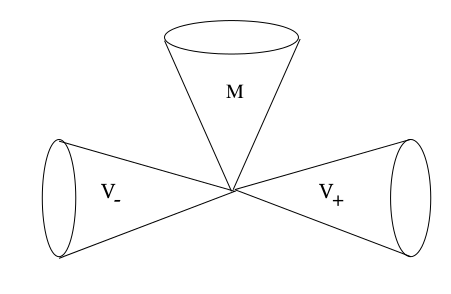
\includegraphics[scale=0.38]{u1_threecones.png}
\caption{Schematic picture of the origin of the moduli space for a $U(1)$ gauge theory.}
\label{fig:u1_origin_cones}
\end{figure}	
\\
Two different chiral fields are needed since near the origin the moduli space shrinks to a point and $V_+ \rightarrow 0$. 
The Higgs branch is not modified by quantum corrections and the mesons can still be used to parametrize it.\\
The charges of the fields under the symmetries are given by
 \begin{equation}
 \begin{array}{ | c | c c c c c |}
 \hline
  & U(1)_R &  U(1)_J & U(1)_A & SU(N_f)_R & SU(N_f)_R \\
 \hline
 Q & 0 & 0  & 1 & N_f & 1  \\  
 \tilde{Q} & 0 & 0  & 1 & 1 & \overbar{N_f}  \\  
   %M & 0 &  0 & 2 & N_f & \overbar{N_f}\\  
   V_{\pm} & N_f & \pm 1  & -N_f & 1  &  1\\
   \hline
 \end{array}
\end{equation}
The symmetries force the superpotential to have the form
\begin{equation}
W = - N_f \left(  V_+ V_- \Det{ (M)} \right)^{\frac{1}{N_f}}
\label{eqn:moduli_space_u1_nfsuperpotential}
\end{equation}
The superpotential is singular at the origin of the moduli space because of the presence of the root, indicating that there are massless degrees of freedom that need to be taken into account.\\
We can give real masses $\bar{m}_i$ ($-\bar{m}_i$) to the quarks $Q_i$ ($\tilde{Q}_i$).
The Higgs branch is parametrised by the diagonal elements of $M^i_{\tilde{i}}$ which intersects the Coulomb branch at $\sigma = \bar{m}_i$.
At every intersection, we have $U(1)$ theory with one flavour.
The coulomb branch is parametrised, at every intersection, by $V_{i,\pm} = e^{\pm \frac{\Phi - \bar{m}_i}{g^2}} $ with a superpotential given by
\begin{equation}
W = - \sum_{i = 1}^{N_f} M^i_i V_{i,+} V_{i,-} + \sum_{i=1}^{N_f - 1} \lambda_i \left(    V_{i,+} V_{i+1,-} - 1\right)
\end{equation}
where $\lambda_i$ are Lagrange multipliers in order the enforce the semiclassical identification  $ V_{i,+} V_{i+1,-} = 1 $.

\begin{figure}[h!]
\centering
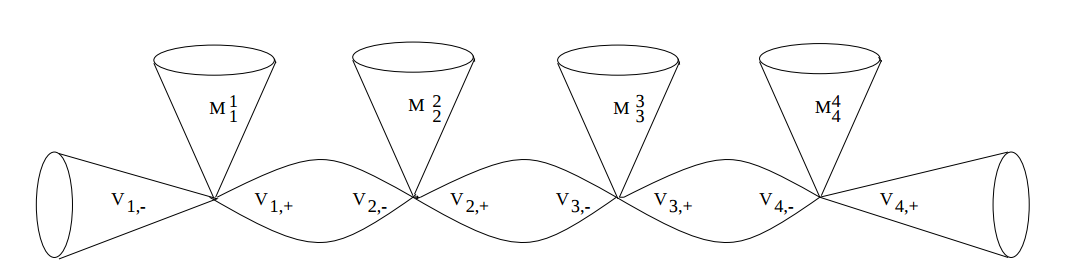
\includegraphics[scale=0.5]{u1_moduli_space_flavours.png}
\caption{Moduli space of vacua for SQED with four flavours}
\end{figure}
















\subsubsection{Moduli spaces for $SU(N_c)$ theories with $N_c >2 $ and with $N_f$ flavours }
\label{sec:modspace_sun_nf}
We will consider a $SU(N_c)$ gauge theory with equal number of $Q$ and $\tilde{Q}$.
%in order to avoid Chern-Simons term. 
The symmetries of the theory are given by the following table
 \begin{equation}
\begin{array}{| c | c c c c c |}
\hline
  & U(1)_R & U(1)_B & U(1)_A & SU(N_f)_L & SU(N_f)_R \\
 \hline
 Q & 0 &1 & 1 & N_f & 1 \\  
 \tilde{Q}& 0 &-1 & 1 &1 & \overbar{N_f}  \\  
   M & 0 & 0 & 2 & N_f & \overbar{N_f}\\  
   Y_{j \neq K} & -2 & 0  & 0 &  1 & 1 \\
   Y_{K} & 2 (N_f -1 ) & 0 & - 2 N_f & 1 & 1 \\
   Y & 2 ( N_f -N_c +1) & 0 & - 2 N_f & 1 & 1 \\
   \hline
\end{array}
\end{equation}
where $Y_j$ are defined as in \eqref{eqn:Y_def_sun_theories} and $Y$ is defined as $Y = \prod_{j=1}^{N_c -1} Y_j \sim e^{ \frac{ \Phi_1 - \Phi_{N_c}  }{g^2}}$.
The VEVs of the adjoint scalar are ordered in such a way that $ \sigma_1 \geq \sigma_2 \geq \dotsc \geq \sigma_{N_c}$. 
The value of $j$ for which $\sigma$ changes sign is called $K$.
In a generic point of the Higgs branch, the gauge group to $SU(N_f -N_c)$ for $N_f <N_c -1 $ and it breaks completely for $N_f \geq N_c - 1$. 
As in four dimensions the Higgs branch is parametrised by mesons and, for $N_f \geq N_c$, by baryons too.
\\
For theories without quarks, instantons generate the Affleck-Harvey-Witten \cite{Affleck:1982as} superpotential
\begin{equation}
W = \sum_{j=1}^{N_c - 1} \frac{1}{Y_j}
\label{eqn:def_AHW_Superpotential_Sun}
\end{equation}
which prohibits the theory to have stable supersymmetric vacua by lifting completely the Coulomb branch.\\
The theory with massless quarks features a superpotential generated by $N_c - 2$ instantons 
\begin{equation}
W_{inst} = \sum_{j \neq K} \frac{1}{Y_j}
\label{eqn:AHW_superpotential}
\end{equation}
which doesn't completely lift the Coulomb branch.
In fact, the following subspace is not lifted by the AHW superpotential \eqref{eqn:def_AHW_Superpotential_Sun}
\begin{equation}
 \sigma_1 > \sigma_2 = \dots = 0 > \sigma_{N_c} = - \sigma_1
 \label{eqn:ahw_subspace_unlifted}
\end{equation}
The last equality holds because we have $\sum_i \sigma_i = 0$ for $SU(N_c)$ gauge group.
\\
The quantum corrected moduli space is different from the classical one and for $N_f < N_c -1 $ the only effective superpotential which is compatible with the symmetries of the theory is given by \cite{Aharony:1997bx}
\begin{equation}
 W_{eff} = (N_c - N_f - 1) ( Y \Det{(M)} ) ^{\frac{1}{N_f - N_c +1}}
\end{equation}
which admits no stable vacuum.\\
For $N_f = N_c - 1 $ the effective superpotential defined above is not defined.
For these values we have a constraint on the moduli space given by \cite{Aharony:1997bx} 
\begin{equation}
Y \Det( M) = 1
\label{eqn:suN-3d-nf-nc-1-vacuum}
\end{equation}
which results in a merging between the Higgs and the Coulomb branch.

For $N_f \geq N_c $, the low-energy description contains baryons.
The quantum moduli space is the same as the semi-classical moduli space and there is a superconformal fixed point at the origin.
In the $N_f = N_c$ case an effective description of the moduli space can be given and the superpotential is \cite{Aharony:1997bx}
\begin{equation}
W = - Y ( \Det{(M)} - B \tilde{B})
\label{eqn:3d_sun_nf__n_c_superpot}
\end{equation}
which forces the theory to flow to a non-trivial fixed point in the infrared.\\
For $N_f >N_c$ an effective description is not known.
\\
The above analysis can be extended to theories with $U(N_c)$ gauge group with $N_f \leq N_c$.
We will discuss the theory with $N_f = N_c$ because the results with lower number of flavours can be obtained by integrating out quarks.\\
The theory with $U(N_c)$ is obtained by gauging the global $U(1)_B$ factor.\\
Given that we have $N_f=N_c$, the superpotential \eqref{eqn:3d_sun_nf__n_c_superpot} from the $SU(N_c)$ part of the group is present and for the $U(1)$ factor we have one flavour given by $X = B \tilde{B}$ 
and chiral fields $V_+ \, , \,V_-$, defined as 
\begin{equation}
V_+ \sim \exp{ \left(  \frac{\Phi_1}{g^2} + i \gamma_1 \right) } \qquad \quad V_- \sim \exp{ \left( \frac{\Phi_{N_c}}{g^2} + i \gamma_{N_c} \right) }
\label{eqn:un_moduli_space_coordinates}
\end{equation}
because the null trace condition does not hold any more.\\
 The $U(1)$ sector has a superpotential given by
 $$ W = - X V_+ V_-$$
As a result, the superpotential for the theory is given by
\begin{equation}
 W = - Y ( \Det{(M)}  - X) - X V_+ V_- 
 \end{equation} 
Integrating out the massive field $Y$  we obtain a superpotential
\begin{equation}
W = -  V_+ V_-  \Det{(M)}
\label{eqn:aharony_dual_description_NcNf}
\end{equation}


















\section{Aharony duality }
One of the first three dimensional dualities was found by Aharony \cite{Aharony:1997gp} and Karch \cite{Karch:1997ux} for theories with gauge group $U(N_c) $ and non-chiral matter in the fundamental representation.
The charges of the fields are given by the following table
\begin{equation}
\begin{array}{ | c | c c c c c |}
\hline
  & U(1)_R & U(1)_A & U(1)_J  & SU(N_f)_L & SU(N_f)_R \\
 \hline
 Q & 0 & 1& 0 & N_f& 1 \\ 
 \tilde{Q} & 0  & 1&0 & 1 & \overbar{N_f}  \\  
   M & 0 & 2 & 0 & 1 & 1 \\ 
  V_{\pm} & N_f - N_c + 1 & - N_f  & \pm 1 &  1 & 1 \\
  \hline
\end{array}
\end{equation}
where $V_{\pm} $ are defined as in the previous section and parametrize the unlifted Coulomb branch.
The R-charges of the quarks have been fixed to zero in order to have the fermion in the multiplet with R-charge $-1$.
The moduli space of this theory was described in the previous section.
\\
The dual theory is a $U(\tilde{N}_c) = U(N_f - N_c) $ gauge theory with $N_f$ flavours $q\, ,\, \tilde{q}$ and with the addition of singlet fields  $M \,,  V_+ \, , V_-$ with the same quantum number of the electric theory. 
The charges are chosen in order to be consistent with a potential $W = M \, q \tilde{q}$ as in four dimensional dualities.\\
The global charges of the theory are given by
\begin{equation}
\begin{array}{ | c | c c c c c | }
\hline
  & U(1)_R & U(1)_A & U(1)_J  & SU(N_f)_L & SU(N_f)_R \\
 \hline
 q & 1 & -1 & 0 & \overbar{N_f} & 1 \\  
 \tilde{q}& 1  & -1 & 0  & 1 & {N_f}  \\  
 \tilde{V}_{\pm} & N_c - N_f -1 & N_f  & \pm 1 &  1 & 1 \\
 \hline
\end{array}
\end{equation}
The magnetic theory features a superpotential of the form
\begin{equation}
W = M^{\tilde{i}}_i q^i \tilde{q}_{\tilde{i}} + V_+ \, \tilde{V}_- + V_- \, \tilde{V}_+
\label{eqn:aharony_mag_superpotential}
\end{equation}
The dual theory now contains the fields $V_+ \, , \, V_-$ which are matched with the coordinate on the Coulomb branch of the electric theory.
Consider that in three dimensions the moduli space contains the Coulomb branch, which wasn't present in four dimensional theories.
The introduction of the monopoles is crucial in order to have the same moduli space between the two theories.\\
The dual theory exists only for $N_f > N_c$. 
Starting with $N_f =N_c + 1$ we obtain a dual theory with $U(1)$ gauge group. Adding a mass term of the form $m M$ in the dual theory breaks the gauge group. After integrating out quarks and $\tilde{V}_{\pm}$ fields we obtain an effective description given only by mesons and $V_{\pm}$ with no other fields.
The superpotential is constrained by symmetries to be of the form 
\begin{equation}
W = - V_+ V_- \Det{(M)}
\end{equation}
We found exactly the dual description of the theory we introduced in \eqref{eqn:aharony_dual_description_NcNf} for the case $N_f =1$.
\\
We can compare the moduli space between the dual theories by looking at specific vacua.
For example, let's consider a point on the Higgs branch in the electric theory with vacuum expectation values of the mesons of rank $N_c$.
The low-energy dual theory associated to such a VEV is a $U(N_f - N_c)$ theory with $N_f - N_c$ massless flavours whose moduli space can be described by a superpotential of the form $W = \tilde{V}_+ \tilde{V}_- \, \Det{( q \tilde{q})} $ since $N_f = \tilde{N}_c$.
\\
The equations of motion resulting from the addition of this term to the superpotential \eqref{eqn:aharony_mag_superpotential} set $V_+ = V_-= 0$, as in the electric theory.\\
%If the VEV of the mesons has rank $N_c -1 $ the original theory is not completely higgsed and the dual theory can be given an effective description through the superpotential $W = \left(  \tilde{V}_+ \tilde{V}_- \, \Det{q \tilde{q}} \right)^{\frac{1}{2}}$ since $N_f = \tilde{N_c} +1$















\section{Kim-Park duality}
Aharony duality can be generalised with the addition of a field in the adjoint representation \cite{Kim:2013cma}.\\
The electric theory contains $N_f$ flavours and a chiral multiplet in the adjoint representation. 
The theory has a superpotential given by $W = tr X^{k+1}$ that fixes the R-charge of the field to $\Delta_X = \frac{2}{k+1}$.
The R-charges of the quarks have been left unconstrained to the generic value $\Delta_Q$.\\
The charges of the fields are given by
\begin{equation}
\begin{array}{ | c | c c c c c |}
\hline
  & SU(N_f)_L & SU(N_f)_R & U(1)_A & U(1)_J  & U(1)_R   \\
 \hline
 Q & N_f & 1& 1 & 0   & \Delta_Q  \\  
 \tilde{Q} & 1 & \overbar{N_f} & 1 & 0 & \Delta_Q      \\  
  X & 1 & 1  & 0 & 0 & \frac{2}{k+1}  \\ 
 v_{j,\pm} & 1  &1   & - N_f & \pm 1 & -N_f (\Delta_Q-1 ) - \frac{2}{k+1} (N_c-1 - j) \\
 \hline
\end{array}
\end{equation}
where $v_{j,\pm}$ with $j=0,\dotsc,k-1$ are the monopole operators dressed with powers of the adjoint field. 
They are defined as \cite{Kim:2013cma}
\begin{equation}
v_{j,\pm} = \Tr{( v_{0,\pm} \, X^{j})}
\label{eqn:3d_mag_monopoles_def}
\end{equation}
where $v_{0,\pm}$ is the bare monopole operator we defined in the previous section in \eqref{eqn:defined_un_cb_coordinates}.\\
To see the reason why there are $k$ different monopoles in this theory we can weakly deform the superpotential to a generic polynomial, as we did in \eqref{eqn:kutasov_deformed_superpotential}.
The effect of this deformation is the breaking of the gauge group $U(N_c)$ in 
\begin{equation}
U(N_c) \; \rightarrow \; U(r_1) \times U(r_2) \times \dots \times U(r_k) \quad \hbox{with} \; \sum r_i = N_c
\end{equation}
Following the same reasoning, in the infrared we find $k$ distinct SQCD sectors with gauge group $U(r_i)$ without adjoint matter, since it has been integrated out.\\
Every sector must have a pair of monopoles since it is a $U(r_i)$ theory, as we have seen in section \ref{sec:modspace_sun_nf}.\\
Going to the limit of vanishing coupling we find that the original theory have $k$ pairs of monopole operators.\\
%%%% DICO perchè son vestiti così


The magnetic theory is a $U(k N_f - N_c)$ gauge theory with $N_f$ dual quarks $(q,\tilde{q})$, adjoint matter $Y$ and singlet fields $(M_j)^{i}_{\tilde{i}}$ and $v_{j,\pm}$. Mesons are constructed from the quarks and the adjoint matter in the electric theory and the $v_{j,\pm}$ are the electric monopole operators.\\
The charges of the fields are given by
\begin{equation}
\begin{array}{ | c | c c c c c | } 
 \hline
  & SU(N_f)_L & SU(N_f)_R & U(1)_A & U(1)_J  & U(1)_R   \\
 \hline
 q & N_f & 1& 1 & 0   & \Delta_q  \\  
 \tilde{q} & 1 & \overbar{N_f} & 1 & 0 & \Delta_q      \\  
  Y & 1 & 1  & 0 & 0 & \frac{2}{k+1}  \\ 
  M_j & N_f & \overbar{N_f} & 2  &  0& 2 \Delta_Q + j \frac{2}{k+1} \\
  v_{j,\pm} & 1  &1   & - N_f & \pm 1 & -N_f (\Delta_Q-1 ) - \frac{2}{k+1} (N_c-1 - j) \\
 \tilde{v}_{j,\pm} & 1  &1   & N_f & \pm 1 & N_f (\Delta_Q-1 ) + \frac{2}{k+1} (N_c + 1 + j) \\
 \hline
\end{array}
\label{tab:kim-park-magnetic}
\end{equation}
The fields $\tilde{v}_{j,\pm}$ are the monopole operators of the magnetic theory and are constructed in the same way of the electric ones.
The charges of the dual quarks and of the adjoint matter are chosen in order to be compatible with a superpotential 
\begin{equation}
W = \Tr{ Y^{k+1}} + \sum_{j=0}^{k-1} M_j \, \tilde{q}\, Y^{k - j - 1} q 
\end{equation}
as Kutasov-Schwimmer duality in four dimensions.\\
The charges of the monopole operators can be calculated by counting their fermion zero modes and are compatible with a superpotential of the form
\begin{equation}
W_{monopoles} = \sum_{j=0}^{k-1} \left(   v_{i,+} \, \tilde{v}_{k-j-1,-} + v_{j,-} \, \tilde{v}_{k-j-1,+} \right)
\label{eqn:kimpark_superpotential_monopoles}
\end{equation}
The duality maps the electric adjoint field with the magnetic one.
Mesons and monopole operators in the electric theory are mapped as singlets in the magnetic one. 